\section{Advancements in digitizer-enabled neutron \tot\ measurements of rare
isotopes}
By applying newly-available digitizer technology to reduce per-event deadtime,
we have advanced a program of isotopic \tot\ 
measurements valuable for constraining the isovector strength of the nuclear potential at positive 
energies. New data have been obtained on \oEight, \niEightFour, \snTwelveFour\ up
to 450 \mega\electronvolt, dramatically expanding the coverage of these nuclei
and laying the groundwork for subsequent optical model analyses. At the same
time, we have identified shortcomings in the digital-signal-processing approach
that must be rectified in future measurements, namely, the uncertainty in the
true analytic deadtime and in the deadtime associated with digitizer buffer
readout to the data acquisition computer. These effects depend on
the proprietary digitizer firmware algorithms used for peak
identification and buffer management, both of which are opaque to the
end user. In an ideal experiment, DPP and raw waveform traces should be collected
in parallel throughout the experiment and compared during data analysis to
pinpoint any weaknesses in the peak-detection algorithm and identify variations in the analytic
deadtime. Due to the ferocious data rate, we could only
collect small snippets of raw waveform data, insufficient for a full
DPP-raw-waveform comparison.
To resolve the discrepancy in our results above 100
\mega\electronvolt\ with those of \cite{Finlay1993} and \cite{Abfalterer2001},
we suggest two types of benchmarking experiments in the future. First is a
two-digitizer experiment: the same detector signals are fed into two
separate time-synchronized digitizers, one running only in DPP mode,
and one running in raw waveform mode. During analysis, a simulated DPP-mode peak sensing
algorithm can be developed, applied to the real raw waveform-mode data, and its
results compared with the real DPP-mode data, clarifying the DPP-mode behavior of
the digitizer firmware. The second experimental setup would use
both a digitizer and analog electronics:
the same signals would be fed both into the digitizer, as
in our experiment, and into analog-electronics logic utilizing a ``looking
period'' (shown in Fig. \ref{AnalogLogic}).

\section{Implications of DOM results}
Our DOM analyses of \oSixEight, \caAughtEight, \niEightFour, \snTwelveFour,
and \pbEight\ have yielded new insight into the validity of the DOM approach
and what experimental data are most needed for improved calculations of
essential structural quantities. Our successful fits of \oSixEight\ show that
even lighter systems (e.g., \cTwelve) may be amenable to a non-local DOM
treatment, providing a bridge between ab initio calculations and
phenomenological optical models. The shape of the imaginary potential
above the Fermi energy is consistent across all our fits and agrees
qualitatively with the state-of-the-art global optical model of \cite{KoningDelaroche}. 
Below the Fermi energy where experimental data is much sparser, we see
significant variation in the shape of the potential between nuclei especially
near the Fermi surface, where the magnitude of the imaginary potential changes
rapidly. This is most conspicuous in the lighter nuclei where a reduced level density
makes a smooth optical potential a poor approximation.
Heavy nuclei have sufficient phase space and level density on both
sides of the Fermi energy that the nuclear potential is largely symmetric near
the Fermi energy, in keeping with the expectations of Mahaux and Sartor \cite{Mahaux1991}.

By comparison to experimentally-measured charge density distributions, we confirm
that significant depletion of s-shell occupation is needed to reproduce the
proton density in the nuclear core. When the binding energy is included in our fits,
we see a significant increase in imaginary strength below -100
\mega\electronvolt, indicating that a significant fraction of the nuclear
binding energy comes a small fraction of nucleons far more deeply bound than
shell models indicate. That a small fraction of nucleons should experience a
very deep potential -- and that the minority nucleon (e.g., protons in \pbEight)
spends more time very deeply bound -- emphasizes how important short-range
correlations are for nuclear binding and the nucleon momentum distribution.

The neutron skins we extract show the central role of shell structure in
determining the neutron skin thickness. To wit, the neutron skin thickness we
extract for \oEight\ (0.21 \femto\meter) appears to be as large or larger than that of
\pbEight\ (0.19 \femto\meter), even though the asymmetry ratio of \pbEight\
(0.212) is almost twice as large as that of \oEight\ (0.111). In light of this
result, we expect that in the N=34 isotone, the filling of the $\nu$ \fSeven\ and \fFive\ subshells
may give $^{52}$Ar and $^{54}$Ca very large neutron skins, potentially even
larger than in even heavier Ar and Ca isotopes. Future experiments at FRIB and other
radioactive beam facilities will probe this region and clarify the relative
importance of the asymmetry ratio, high-spin intruder subshells in determining
the neutron distribution near the dripline.
\begin{figure}[tb]
    \centering
    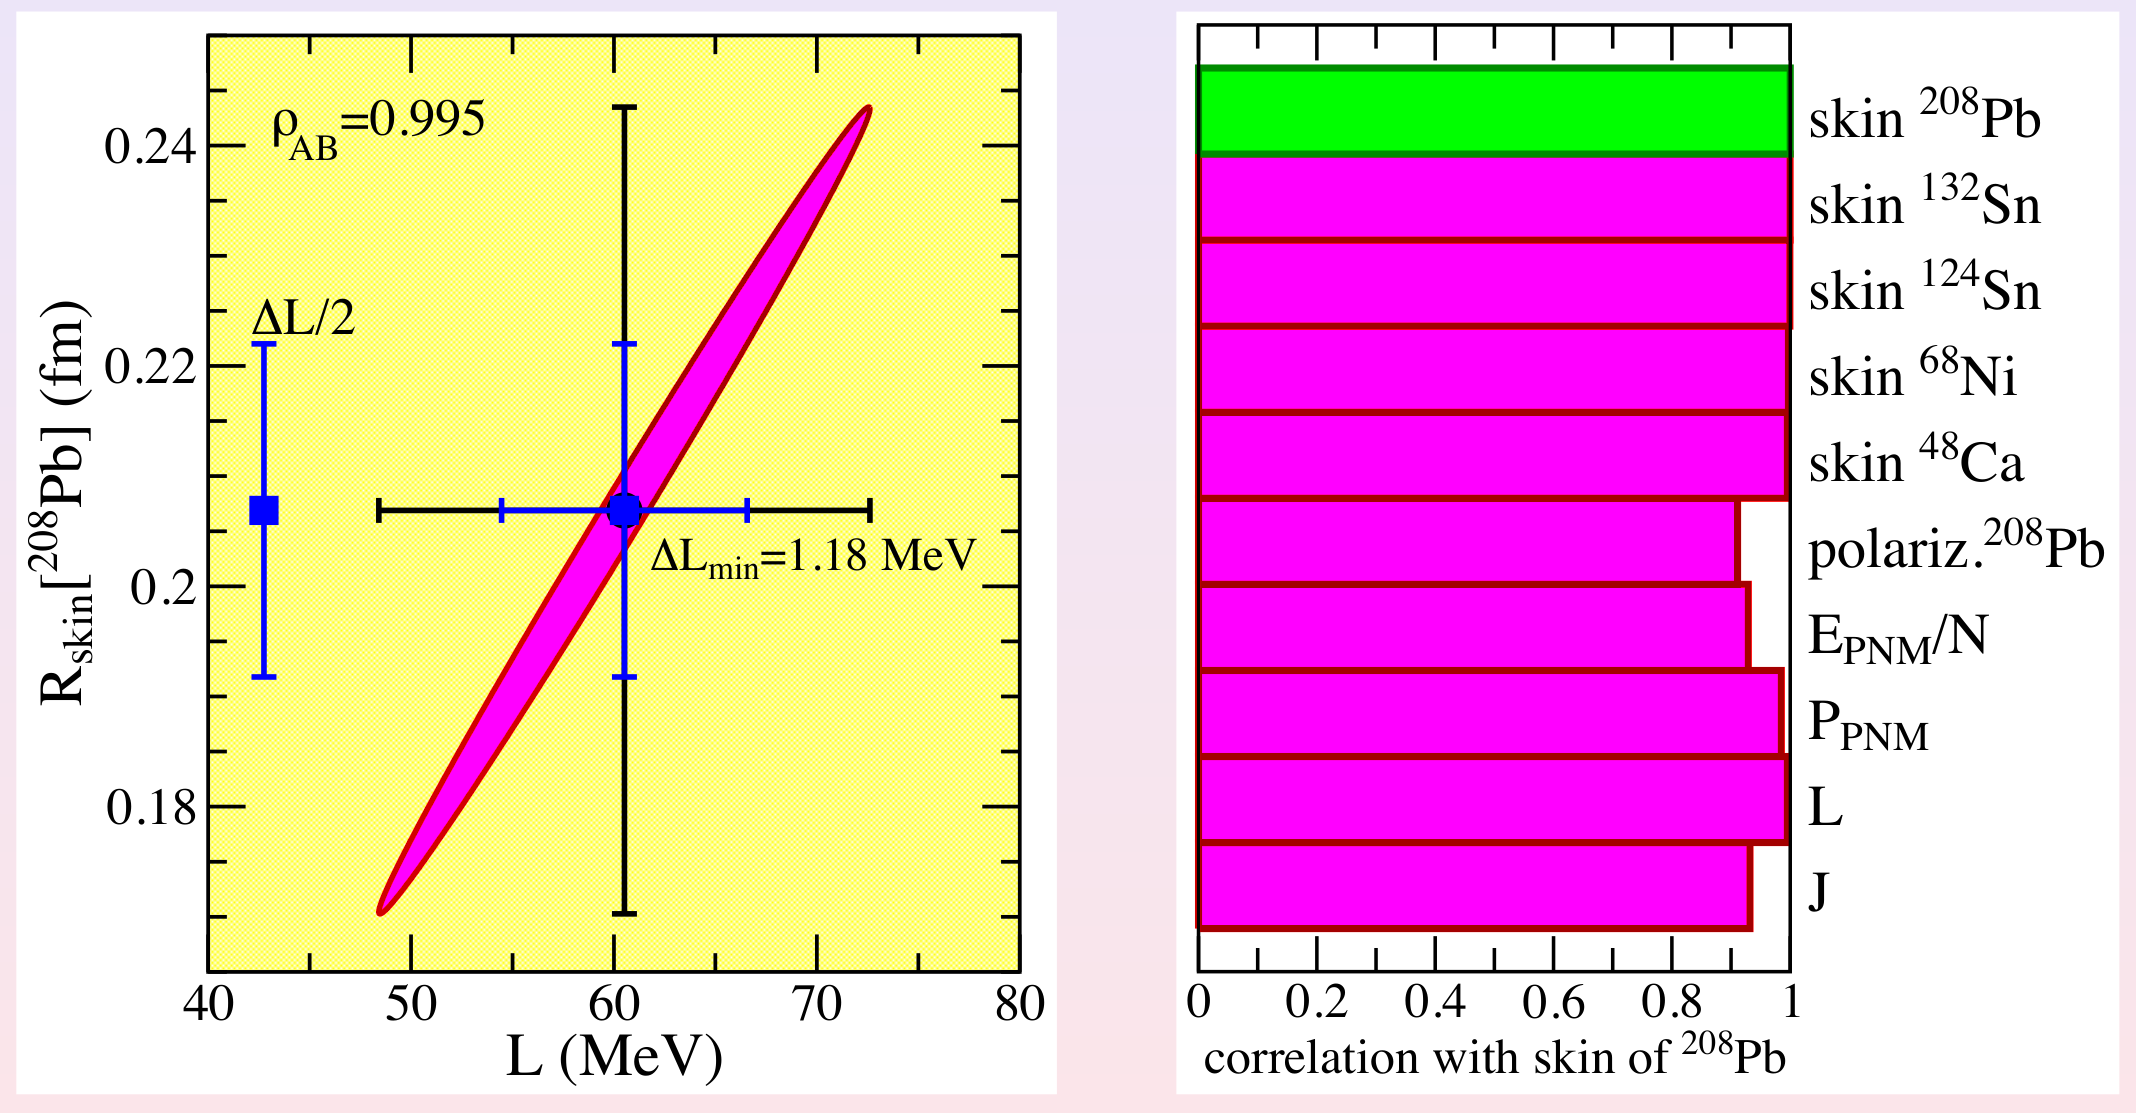
\includegraphics[width=0.9\textwidth]{figures/PiekarewiczPb208SkinCorrelation.png}
    \caption[Correlation between the neutron skin of \pbEight\ and several nuclear structure
    observables]
    {
        Correlation between the neutron skin of \pbEight\ and several nuclear structure observables,
        per a relativistic mean-field calculation with the FSUGold interaction
        conducted by J. Piekarewicz. Many
        mean-field models recover a very strong correlation between the size of the
        neutron skin of several neutron rich nuclides and the density-dependence of the symmetry
        energy, $L$. Figure used with permission.
    }
    \label{Pb208Correlation}
\end{figure}
In relativistic and non-relativistic mean-field models, the neutron skin,
electric dipole polarizability, and dipole resonances of neutron-rich nuclei are
shown to be tightly correlated with the density-dependence of the symmetry
energy, $L$.
\begin{wrapfigure}{i}{0.5\textwidth}
    \centering
    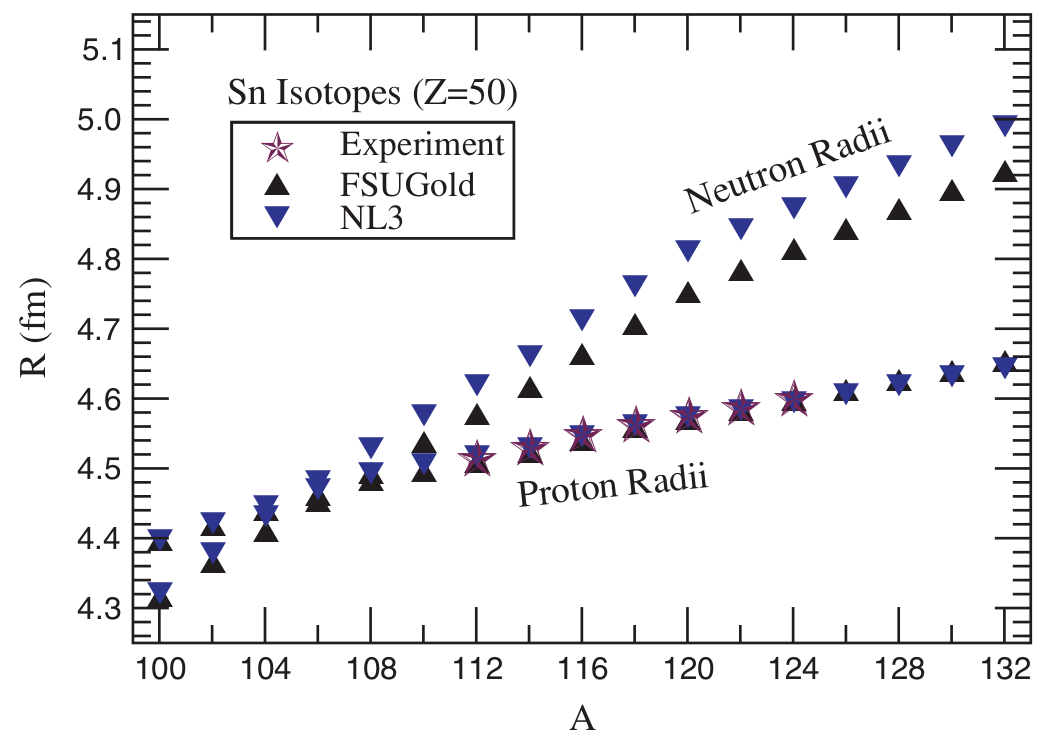
\includegraphics[width=0.48\textwidth]{figures/Piekarewicz2006SnIsotopes.png}
    \caption[Proton and neutron RMS radii in the Sn isotopes computed with FSUGold and NL3
    interactions]
    {
        Proton and neutron RMS radii in the Sn isotopes computed in a relativistic mean-field
        approximation using the FSUGold and NL3 parameter sets, with experimental data for comparison.
        Figure and caption used with permission from \cite{Piekarewicz2006}.
    }
    \label{Piekarewicz2006SnIsotopes}
\end{wrapfigure}
For example, Fig. \ref{Pb208Correlation} shows the results of a covariance
analysis on a variety of observative quantities calculated by a relativistic mean-field model 
employing an FSUGold interaction \cite{Fattoyev2012}. The neutron
skin for \pbEight\ generated by our fit is in good agreement with this model.
However, another treatment that uses the same interaction
\cite{Piekarewicz2006} gives a neutron skin for \snFour\ of roughly 0.22
\femto\meter\ (see Fig. \ref{Piekarewicz2006SnIsotopes}), much larger than the
[insert final \snFour\ neutron skin] \femto\meter\ generated by our fit.
Understanding the model-dependence of these predictions, both from relativistic mean-field
approaches and from the DOM, is critical for making progress on constraining
$L$. As has been pointed out by others, a multi-pronged approach 
is warranted: electroweak measurements like PREX \cite{Horowitz2014}, comparison of
charge radii in mirror nuclei \cite{Brown2017}, modeling of dipole
polarizability \cite{Piekarewicz2006}, and multi-messenger astrophysical
measurements on neutron stars. Given the new results presented in this work, we
hope to add theoretical predictions from the DOM to the mix.

\section{Topics for Future Study}
Given the advances and limitations of this work, we can identify several
additional avenues of research worth pursuing.
Besides the digitizer benchmarking experiments described earlier
in this chapter, \tot\ measurements on the stable Fe and Cd isotopes would
supplement our Ni and Sn isotope studies and provide much-needed information
about optical-potential isovector dependence outside closed proton shells.
Data for \tot\ on the intermediate stable isotopes $^{114,116,118,120,122}$Sn
would improve optical-model extrapolations to $^{100}$Sn and $^{132}$Sn,
both of which are valuable for testing shell-model validity near the driplines.
We reiterate the importance of new proton \rxn\
studies across the chart of nuclides, particularly on closed-shell isotope and isotone
chains. 

A major drawback of the DOM implementation presented in this work is
the lack of covariance analysis of DOM parameters. Without theoretical error
bars associated both with uncertainty in the experimental data used and in the
DOM's parameteric forms, comparisons between the DOM and other models cannot be
complete. A first step toward this goal is publication of the DOM codebase, a
priority under contemplation within our group.
